% AEJ-Article.tex for AEA last revised 22 June 2011
\documentclass[AEJ]{AEA}

%%%%%% NOTE FROM OVERLEAF: The mathtime package is no longer publicly available nor distributed. We recommend using a different font package e.g. mathptmx if you'd like to use a Times font.
% \usepackage{mathptmx}

% The mathtime package uses a Times font instead of Computer Modern.
% Uncomment the line below if you wish to use the mathtime package:
%\usepackage[cmbold]{mathtime}
% Note that miktex, by default, configures the mathtime package to use commercial fonts
% which you may not have. If you would like to use mathtime but you are seeing error
% messages about missing fonts (mtex.pfb, mtsy.pfb, or rmtmi.pfb) then please see
% the technical support document at http://www.aeaweb.org/templates/technical_support.pdf
% for instructions on fixing this problem.

% Note: you may use either harvard or natbib (but not both) to provide a wider
% variety of citation commands than latex supports natively. See below.

% Uncomment the next line to use the natbib package with bibtex 
\usepackage{natbib}
\usepackage{hyperref}
\usepackage{acronym}
\usepackage[names]{xcolor}
\usepackage{graphicx}
\usepackage{csvsimple}
% Uncomment the next line to use the harvard package with bibtex
%\usepackage[abbr]{harvard}
\usepackage{etoolbox}
\newtoggle{fancy}
\togglefalse{fancy}

\usepackage{xspace}
% to adjust floats
\usepackage{placeins}
% to read the table
\usepackage{csvsimple}
\usepackage{longtable}

\usepackage{textcomp}

\iftoggle{fancy}{
\usepackage[most]{tcolorbox}
\usetikzlibrary{calc}
\tcbset{
	toplength/.store in={\tcbcornerruletoplength},
	leftlength/.store in={\tcbcornerruleleftlength},
	toplength=3cm,
	leftlength=2cm,
	bottomlength/.store in={\tcbcornerrulebottomlength},
	rightlength/.store in={\tcbcornerrulerightlength},
	bottomlength=3cm,
	rightlength=2cm,
	cornerruleshift/.store in={\tcbcornerruleshift},
	cornerruleshift=1pt,
	topcornercolor/.store in={\tcbtopcornercolor},
	bottomcornercolor/.store in={\tcbbottomcornercolor},
	topcornercolor=green!40!blue,
	bottomcornercolor=blue!40!green,
}

\newtcolorbox{cornerbox}[1][]{%
	enhanced jigsaw,
	sharp corners,
	boxrule=0pt,
	underlay={
		\coordinate (topend) at ($(frame.north west) + (0:\tcbcornerruletoplength)$);
		\coordinate (leftend) at ($(frame.north west) - (90:\tcbcornerruleleftlength)$);
		\coordinate (bottomend) at ($(frame.south east) - (0:\tcbcornerrulebottomlength)$);
		\coordinate (rightend) at ($(frame.south east) + (90:\tcbcornerrulerightlength)$);
		\draw[line width=2pt,\tcbtopcornercolor] ([xshift=-\tcbcornerruleshift]leftend) -- ([shift={(-\tcbcornerruleshift,\tcbcornerruleshift)}]frame.north west) -- ([shift={(-\tcbcornerruleshift,\tcbcornerruleshift)}] topend);
		\draw[line width=2pt,\tcbbottomcornercolor] ([xshift=\tcbcornerruleshift]rightend) -- ([shift={(\tcbcornerruleshift,-\tcbcornerruleshift)}]frame.south east) -- ([shift={(-\tcbcornerruleshift,-\tcbcornerruleshift)}] bottomend);
	},
	#1,
}
}{}

% This command determines the leading (vertical space between lines) in draft mode
% with 1.5 corresponding to "double" spacing.
\draftSpacing{1.5}

%% make somewhat tigher enumeration environments
\usepackage{enumitem}
\setlist[enumerate]{itemsep=0pt,parsep=0pt,topsep=1pt}
\setlist[itemize]{itemsep=0pt,parsep=0pt}

%% Acronyms
\acrodef{AEA}{American Economic Association}
\acrodef{DOI}{Digital Object Identifier}
\acrodef{FAIR}{Findable, Accessible, Interoperable, Re-usable}
\acrodef{PSID}{Panel Study of Income Dynamics}
\acrodef{HRS}{Health and Retirement Study}
\acrodef{RCT}{randomized control trial}

% reset colors
\definecolor{darkblue}{rgb}{0 0 255}
\hypersetup{colorlinks,breaklinks,citecolor=darkblue,linkcolor=darkblue,urlcolor=darkblue}

% Different ways to cite URLS
%\newcommand{\urlcite}[2]{\href{#1}{#2}
\newcommand{\urlcite}[2]{#2\footnote{\url{#1}}}

\begin{document}

\title{Report for 2018 by the AEA Data Editor }
\shortTitle{Report by Data Editor}
\author{Lars Vilhuber\thanks{%
Vilhuber: Cornell University, lars.vilhuber@cornell.edu.}}
\date{\today}
\pubMonth{Month}
\pubYear{Year}
\pubVolume{Vol}
\pubIssue{Issue}
\JEL{}
\Keywords{reproducibility; replicability; science of science}




\maketitle


The purpose of scientific publishing is the dissemination of robust research findings, exposing them to the scrutiny of peers. Key to this endeavor is documenting the provenance of those findings. For theoretical articles, these are the proofs of theorems and the like that the authors provide. For empirical articles, the foundations on which the findings reside are external to the article, and often to the journal, in which they are published. Many scientists,  journals, learned societies, and funding agencies have called for greater transparency of research practices, and more assurance that published research is reproducible \citep{Stodden2016-uc,Fuentes2016-wz,Moffitt2016-wl,Camerer2016-kl,Bollen2015-vb,Joskow2015-hd,ChristensenTransparencyReproducibilityCredibility2018}. Our scientific community faces  increasingly complex issues of privacy and confidentiality that prevent ``open'' access to those same sources \citep{Anderson12009,abowdschmutte.aer.2018}. Large and private databases (often both at the same time) are being used to analyze economic phenomena, with subsequent publications \citep{BakerWagePolicyFirm1994,LazearAm.Econ.Rev.2000,BaileySocialConnectednessMeasurement2018,Chen2017,HallILRReview2018}, yet few such data are available for replication exercises \cite{JengAm.Econ.Rev.2016}. To ensure the credibility of the scientific endeavor, transparency of the methods and data used are critical. Various studies have shown that too few studies are (easily) reproducible \citep{McCullough2007-zx,McCullough2006-cz,AndersonJ.Econ.Methodol.2008,AndersonFed.ReserveBankStLouisRev.1994}. There is a need to properly cite the digital inputs to our published output and to properly curate those inputs.  

In January 2018, I was appointed as the first Data Editor of the American Economic Association, with the mission to ``design  and  oversee  the  AEA  journals’  strategy for archiving and curating research data and promoting  reproducible  research'' \citep{10.1257/pandp.108.745}. This first report by a Data Editor describes my efforts over the past year to advance  that mission. It also highlights some of the short- and medium-term changes that economists might expect when publishing their research.\footnote{A variety of replication concepts have been defined in economics \citep{Hamermesh2007,ClemensJ.Econ.Surv.2017}. In this article, we adopt the definitions articulated by \citet{Bollen2015-vb}, among others. \textit{Reproducibility}  refers to ``the ability [$\dots$] to duplicate the results of a prior study using the same materials and procedures as were used by the original investigator,'' and is related to the ``narrow" sense of replication of \cite{Pesaran2003}. Use of the ``same procedures'' may imply using the same computer code or re-implementing the statistical procedures in a different software package. \cite{Hamermesh2007} calls this ``pure replication". \citet[p. 942]{ChristensenTransparencyReproducibilityCredibility2018} argue that this is the ``basic standard [that] should be expected of all published economics research, and hope this expectation is universal among researchers.'' \textit{Replicability} refers to ``the ability of a researcher to duplicate the results of a prior study if the same procedures are followed but new data are collected'' \citep[ ``wider'' sense of replication]{Pesaran2003}, while \textit{generalizability} refers to the extension of the scientific findings to other populations, contexts, and time frames, perhaps using different methods \citep[ ``scientific replication'']{Hamermesh2017}}


\section{The current environment}

The \ac{AEA}'s data and code posting policy \citep{American_Economic_Association2008-az}, as well as that of other societies and journals, are a reaction to earlier calls to increase transparency \citep{McCullough2006-cz,AndersonJ.Econ.Methodol.2008}, and are intended to create a minimal framework from which to replicate empirical findings, by requiring the data and code to be available to others. In practice, enough reproduction and replication attempts fail \citep{CamererScience2016,Chang2015-dl,ChangAm.Econ.Rev.2017}, not just in economics \citep{Baker2015-sh,Collaboration2015-ev} (I will comment on our own efforts later). It remains an open question who should be tasked with conducting a ``replication'' in the first place - should the editorial team verify reproducibility during the editorial process \citep{JacobyInsideHigherEd2017}, should the referees be able to do this, or should they be required to do this? Or should the readers of the articles, and the broader scientific community, attest to the replicability and ultimately the generalizability of the findings \citep{Hamermesh2017}? Related is the question whether  enough replications are being published \citep{BerryAm.Econ.Rev.2017,Burman2010-ng,Coffman2017-si,Duvendack2017-js,Hoffler-LibMag.2017}.

Very few journals have implemented verification of submitted code and data during the editorial process. In political science, the American Journal of Political Science in collaboration with the Odum Institute for Research in Social Science \citep{Christian2018} has been conducting data curation and code verification. The Journal of the American Statistical Association performs a ``broad evaluation of quality and potential for usability of the code and data'' since 2016 \citep{Stodden2016-uc}.

%%%% DATA ARCHIVE LISTS
%highlight the verification on data archives \citep{Open_Science_Framework2017-zc}, maintain lists of acceptable third-party repositories,%
%\footnote{Nature Scientific Data maintains a list for its journals \citep{Nature_Scientific_Data2016-hl}, and other institutions (CoreTrustSeal, FAIRsharing) have as their primary purpose to perform this kind of vetting.} 
%and interlink with collaborating repositories to highlight authors' (and repositories') contributions to the data component of a scholarly work.%
%\footnote{Elsevier interlinks, for instance, with ICPSR, highlighting the use of a repository on the article's web page.}

%%% EDUCATION
%Outside of journals, several projects are working to educate the community to incorporate principles of reproducibility and traceability into their workflow.%
%\footnote{Open Science Framework, Project TIER, BITSS are just a few of those active in that field \citep{Gentzkow2014-va,Wilson2016-bt}.}

No journal currently does an adequate job of providing information about restricted-access data.\footnote{Elsevier journals have experimented with "Data Descriptions", but while the form is machine-readable, it is essentially free-form text, and checking the box "confidential data" essentially stops the process of filling in any information.} This is not only the fault of the journals: Most restricted-access data centers do not provide structured information about existence, modalities of access, or even data landing pages for the datasets they provide access to.%
\footnote{Restricted-access data hosted on ICPSR and possibly Harvard Dataverse are notable exceptions.} 
None of these solutions are widespread, and standards are only now being developed.


%
\begin{cornerbox}
In the summer of 2018, I had the privilege of contributing a white paper to the Committee on Reproducibility and Replicability in Science of the National Academies of Science on the history and state of reproducibility in economics. In many sciences, new preprint services have emerged within the last two years, e.g., \href{https://psyarxiv.com/}{PsyArXiv}. These are considered to be part of the broader move to greater research transparency. While writing the white paper, I pointed out that this kind of pre-publication exchange has long been the norm in economics. The first National Bureau of Economic Research (NBER) working paper, one of the most prestigious working paper series in economics, was published (in paper form) in 1973 \citep{WelchEducationInformationEfficiency1973}. By the early 1990s, there was a wide variety of such working paper series, typically provided by academic departments and research institutions. Since grey literature at the time was not cataloged or indexed by most bibliographic indexes, a distinct effort to identify both working papers and the novel electronic versions grew from modest beginnings in 1992 at Université de Montréal and elsewhere into what is today known as the Research Papers in Economics (RePEc) network, a “collaborative effort by hundreds of volunteers in 99 countries” \citep{RePEcResearchPapers,KrichelEconomicsOpenBibliographic2009,Batiz-Lazobriefbusinesshistory2012}. The initial index was split into electronic (WoPEc) \citep{KrichelWoPEcElectronicWorking1997}  and printed working papers (BibEc) \citep{KrichelEconomicsOpenBibliographic2009,CruzCatalogingEconomicsPreprints2000}, testimony to the prevalence of the exchange of scientific research in semi-organized ways.  In 1997, BibEc counted 34,000 working papers from 368 working paper series (30). RePEc today has data from around 4,600 working paper series and claims about 2.5 million full-text (free) research items, provided in a decentralized fashion by about 2,000 archives (31). These items not only include traditional research papers, but also, since 1994, computer code (32–34). 
\end{cornerbox}

\section{The Mission, if You Choose to Accept It}
With the mission outlined above in mind, the Data Editor's long-term tasks are
\begin{enumerate}
	\item Elaborate a data and code availability policy that is modern, responsive, and imposes the lowest burden on authors and readers that is commensurate with the overall goals;
	\item Creating technical, human, and organizational infrastructure at the AEA journals to support all aspects of implementing the data and code availability policy;
	\item Working with other providers of scientific infrastructure to improve support for documenting provenance and replicability;
	\item Working with the economics community to enhance and broaden education on replicable science;
	\item Conducting research and participating in experiments in the intersection of publication, replication, and provenance documentation
\end{enumerate}
In particular, a revised data and code posting policy should maximize credibility and trustworthiness of research findings, and address the following goals: 
\begin{enumerate}
	\item to encourage and reward incorporating basic principles of replicability into researchers' workflow;
	\item to prioritize linking to existing data and code repositories, as the primary mechanism of providing source materials, with a journal-sanctioned repository as a fall-back archive;
	\item to require and facilitate proper documentation of  restricted-access data;
	\item to enforce a limited measure of verification;
	\item balance the previous goals with the need to \textit{reduce} the burden on authors, not increase it. 
\end{enumerate}

\section{Implementing improved transparency of research}
In the first year, we have moved a few tasks forward, though the visible impact on the Association's journals or practices is yet to come. In this section, I lay out both vision, actions, and plans for various goals and tasks. 


\FloatBarrier

\subsection{Task 1: Improved data and code availability policy}
A modern data and code availability policy should support both reproducibility and replicability, by supporting accurate and transparent description of the provenance of the scientific results. In particular, a functional implementation of those concepts suggests that both data and code need to be subject to the \ac{FAIR} principles \citep{FORCE11FAIRDATAPRINCIPLES}: findable, accessible, interoperable, and re-usable. In this context, we interpret the ``interoperability'' of code as ``code that works, and the workings of which are comprehensible by a third party.'' Furthermore, this should be true for \textit{all} data and code, not just code that is open-source and data that is open-access.

\paragraph{Replacing ZIP files} Under this goal, we are working to abolish, or reduce the recourse to, journal-specific ``supplementary materials'' as the primary repository of data and code. As currently implemented at most journals, including the \ac{AEA}'s journals, ``supplementary materials'' are packaged as ZIP files and attached to a web page. Provided in this way, they lack findability, proper citability as first-class objects, and are somewhat opaque. 
To replace such supplementary materials, we are laying the groundwork in three ways. 

\paragraph{Creating the AEA Data and Code Archive} First, we will replace the ZIP files with deposit at a proper data archive, the ``AEA Data and Code Archive.'' The archive will display the full contents of the materials as deposited by authors in the past, without the need to download ZIP files. The archive will be searchable, by JEL codes, keywords, and other characteristics of the data. The materials will receive their own citable \ac{DOI}. Through the \ac{DOI} registrars, we automatically leverage the ability to link and associate the archives with their original articles, but also any other articles that use and cite the data, such as replication articles. Several other economics journals (Quarterly Journal of Economics, the Review of Economics and Statistics) already have similar archives. \textbf{We are currently finalizing contract terms and addressing technical improvements with such a data archive, and expect a decision to be made in time for the Meetings, and the repository to be available for new deposits in 2019Q2.} All historical data supplements will be migrated to the ``AEA Data and Code Archive'' as well, with the \textbf{migration expected to be completed by 2019Q3}.

\paragraph{Allowing third-party repositories} However, if replicability is truly part of the research scientist's workflow, then by the time she submits an article to any journal, the intermediate and final data products as well as the code used for an article have already been deposited at appropriate repositories and archives, albeit in intermediate form. If all such repositories and archives are of sufficient quality, then the additional deposit at a journal is duplicative at best, and perturbative to the provenance chain at worst. The right solution is to reference those other repositories, not copy them.%
\footnote{I note here that some materials associated with the Association's journals have sometimes been deposited at sites such as personal websites, \urlcite{https://github.com}{Github.com}, \urlcite{https://drive.google.com}{Google Drive}, \urlcite{https://dropbox.com}{Dropbox}, and others. These sites are not \textit{considered} data archives, for two key reasons. For one, however unlikely it may seem, these commercial companies are ephemerous, and do not have data preservation as a primary mission. More importantly, users who keep data on these sites can delete the data at any time, for any reason, possibly simply because they did not pay their monthly or annual fee. Such practices are incompatible with proper data curation standards. }
Such a policy is already standard practice in some other domains and publishing platforms (some \urlcite{https://www.springernature.com/gp/authors/research-data-policy/data-policy-types/}{Springer Nature} journals, \urlcite{https://f1000research.com/for-authors/data-guidelines}{F1000 Research}, geosciences).

We will therefore allow authors to keep their supporting materials (data, code) at third-party repositories, as long as those repositories satisfy certain criteria in terms of accessibility and preservation. In particular, this policy will allow us to treat public-use data available through repositories such as \urlcite{https://icpsr.org}{ICPSR} symmetrically with restricted access data curated by survey institutes such as the confidential geodata at the \ac{PSID}, national statistical offices such as the U.S. Census Bureau or Statistics Norway, private-sector research institutes such as the \urlcite{http://www.privatecapitalresearchinstitute.org/}{Private Capital Research Institute}, or private companies such as \urlcite{https://twitter.com}{Twitter} or \urlcite{https://uber.com}{Uber}, as long as objective criteria in terms of \textit{data curation} and \textit{accessibility} are met. If authors do not have access to such an archive, or have not adopted replicable workflows that incorporate data curation, then they will continue to deposit their data and code in the ``AEA Data and Code Archive.'' This new policy will be implemented in parallel with the deployment of the ``AEA Data and Code Archive.''

\paragraph{Transparent method to describe all data and code} Finally, to  support to third-party repositories, we are developing a \textit{data description standard} (in the terms of the trade, a ``metadata schema'') to accurately and completely describe all materials related to a published article, including their access and preservation policies. The data description standard will be accompanied by  tools to support this schema for authors and journal websites.\footnote{A paper describing the schema is scheduled to be presented at the International Digital Curation Conference (IDCC) in February 2019 and is currently being reviewed at the International Journal of Digital Curation} 
The goal of the schema and tools is to move away from idiosyncratic ways to describe and name the data, where to find data, and how to access the data. The ultimate result of implementing the schema will be to provide a more consistent way to display such information within articles or on journal web pages, provide such information in a machine-readable way, and to efficiently leverage the existing metadata that is already provided by numerous data archives. Furthermore, this schema will be implemented as an \textit{information package} that data archives of all kinds can provide to users of their data, and which researchers can share and re-use. The information package is explicitly designed to handle both public-use data archives with well-defined \ac{DOI}, access policies (simple download!), and preservation policies, as well as repositories of restricted-access data without persistent (public) identifiers, complex access policies with myriad rules, and hidden preservation policies. If the data provider does not provide the information package, the author will be able to fill out such a package on her own. I expect this to be a net reduction in time and effort for authors who already describe their data, and to be an increase in work only for those that do not provide complete descriptions of data provenance. In particular authors who use restricted-access data should see a large reduction in the time needed to describe their data access. 

The schema and tools are currently being developed and peer-reviewed, and are expected to be tested  internally in 2019. Conditional on satisfactory performance both for journal managers and users, we plan to deploy it more widely in 2020. 

I emphasize the term ``standard'' used above - our goal is not simply to have a schema of use for the Association's journals, but rather, to allow authors to use the data description we are developing at any journal, not just those published by the Association. We have already reached out to some journals and publishing platforms (see below), and will continue to do so in the next year. 

\paragraph{Timing}
We expect to ask for the \textit{information package} quite early in the submission process, possibly at the same time as manuscript submission itself. In the case of third-party archives, we also expect that authors will have deposited their materials before submission, but no later than the time they receive a revise-and-resubmit. All information will be verified prior to acceptance, rather than prior to publication, as is the case right now. However, we do not expect of authors that the data or code itself be made public prior to publication of the article. 


\paragraph{Visible changes} 
On the AEA's journal websites, the links to ``supplementary'' materials will initially appear to be the same (although pointing to the new locations), but future enhancements will allow for greater visibility or transparency of the associated materials. 
%
Authors submitting their work to the AEA journals will be affected in several ways. First, those authors who already deposit their (open access) code and data at known repositories will not have to do so again - a simple reference (and citation!) of the previously archived materials is sufficient. Authors who use data provided through institutional providers (\ac{PSID}, \ac{HRS}, the U.S. Census Bureau, and international equivalents), and who in some cases cannot deposit the data, will also reference the persistent location where they obtained their data from, and where others can do so as well. In the case of restricted-access, a better description of access procedures will be requested from authors, who in turn should ask their data providers to provide such procedural descriptions, in the form of web pages and (persistent and citable) documents. Once the data description standard mentioned above is available, the information provided by data providers will be captured in that form, and through a web-based tool. 

\FloatBarrier
\section{Task 2: Creating infrastructure at the AEA journals}

\paragraph{Pre-publication verification of reproducibility} One of the key findings of the recent literature has been that code provided by authors, even when deposited at journal as supplementary materials, may not always yield the advertised outcomes \citep{Chang2015-dl,ChangAm.Econ.Rev.2017,Hoeffler2017a}. To that end, we will reinforce the data and code availability policies above by conducting pre-publication verification of code reproducibility. To our knowledge, this has been systematically done only at the American Journal of Political Science \citep{Christian2018}, though the AJPS also does significant data curation tasks for the authors.

The sizeable challenge is how to conduct such pre-publication verification without unduly delaying the editorial workflow. \cite{Christian2018} report lengthy delays between acceptance and publication due to the combination of data curation and code verification. Several factors lead us to think that this is feasible.

For the past 4 years, I have been running a Replication Lab at Cornell with mostly undergraduates. As part of a summer activity (since Fall 2018 also during classes), students download articles and their supplemental data packages from the AEA website, and attempt to reproduce them (``post-publication verification''). The initial focus was on a complete census of the AEJ:AE, but since my appointment in January 2018, the focus has been broadened to AEJ:Macro, AEJ:Micro, and to some extent the other AEA journals. As of December 2018, about 700 articles have been assessed, and about 430 reproduction attempts have been conducted 
%%%
%%%
(a detailed report is being prepared as these lines are being written, and will be available by late December 2018). 

While we have not attempted to measure exact hourly productivity measures, we have some approximate numbers. Over a certain time period in the Summer of 2018, 10 students worked 774 hours. During that time, they assessed 147 articles, attempted 108 replications, and succeeded 49 of those. Thus, 5 students working each a 20-hour workweek can process 20 articles per week, and about 13 reproductions attempted. Note however that these numbers are not representative of all journals. All AEJ:AE articles have an empirical component, in contrast to most other journals. On the other hand, there may be systematic differences in the complexity of the analyses reported in the AEJ:AE relative to other journals. Nevertheless, we believe that an appropriately trained student lab can handle many if not most of the required reproduction attempts.

Second, the variety of software is relatively small. Figure~\ref{fig:aer_programs_by_year} shows the distribution of software in two different samples. Panel (a) identifies software usage in the AER, identified by parsing file extensions in the ZIP archives on the AEA website. Panel (b) identifies software in the AEJ:AE as assessed by the Cornell Replication Lab. Economists in general make heavy use of Stata, with a significant fraction using Matlab. In general, the Cornell Replication Lab had to assign a graduate student (or faculty member) for non-standard software (Gauss, Fortran, etc.), but only very rarely.

\begin{figure}
    \centering
    \begin{tabular}{p{0.45\textwidth}p{0.45\textwidth}}
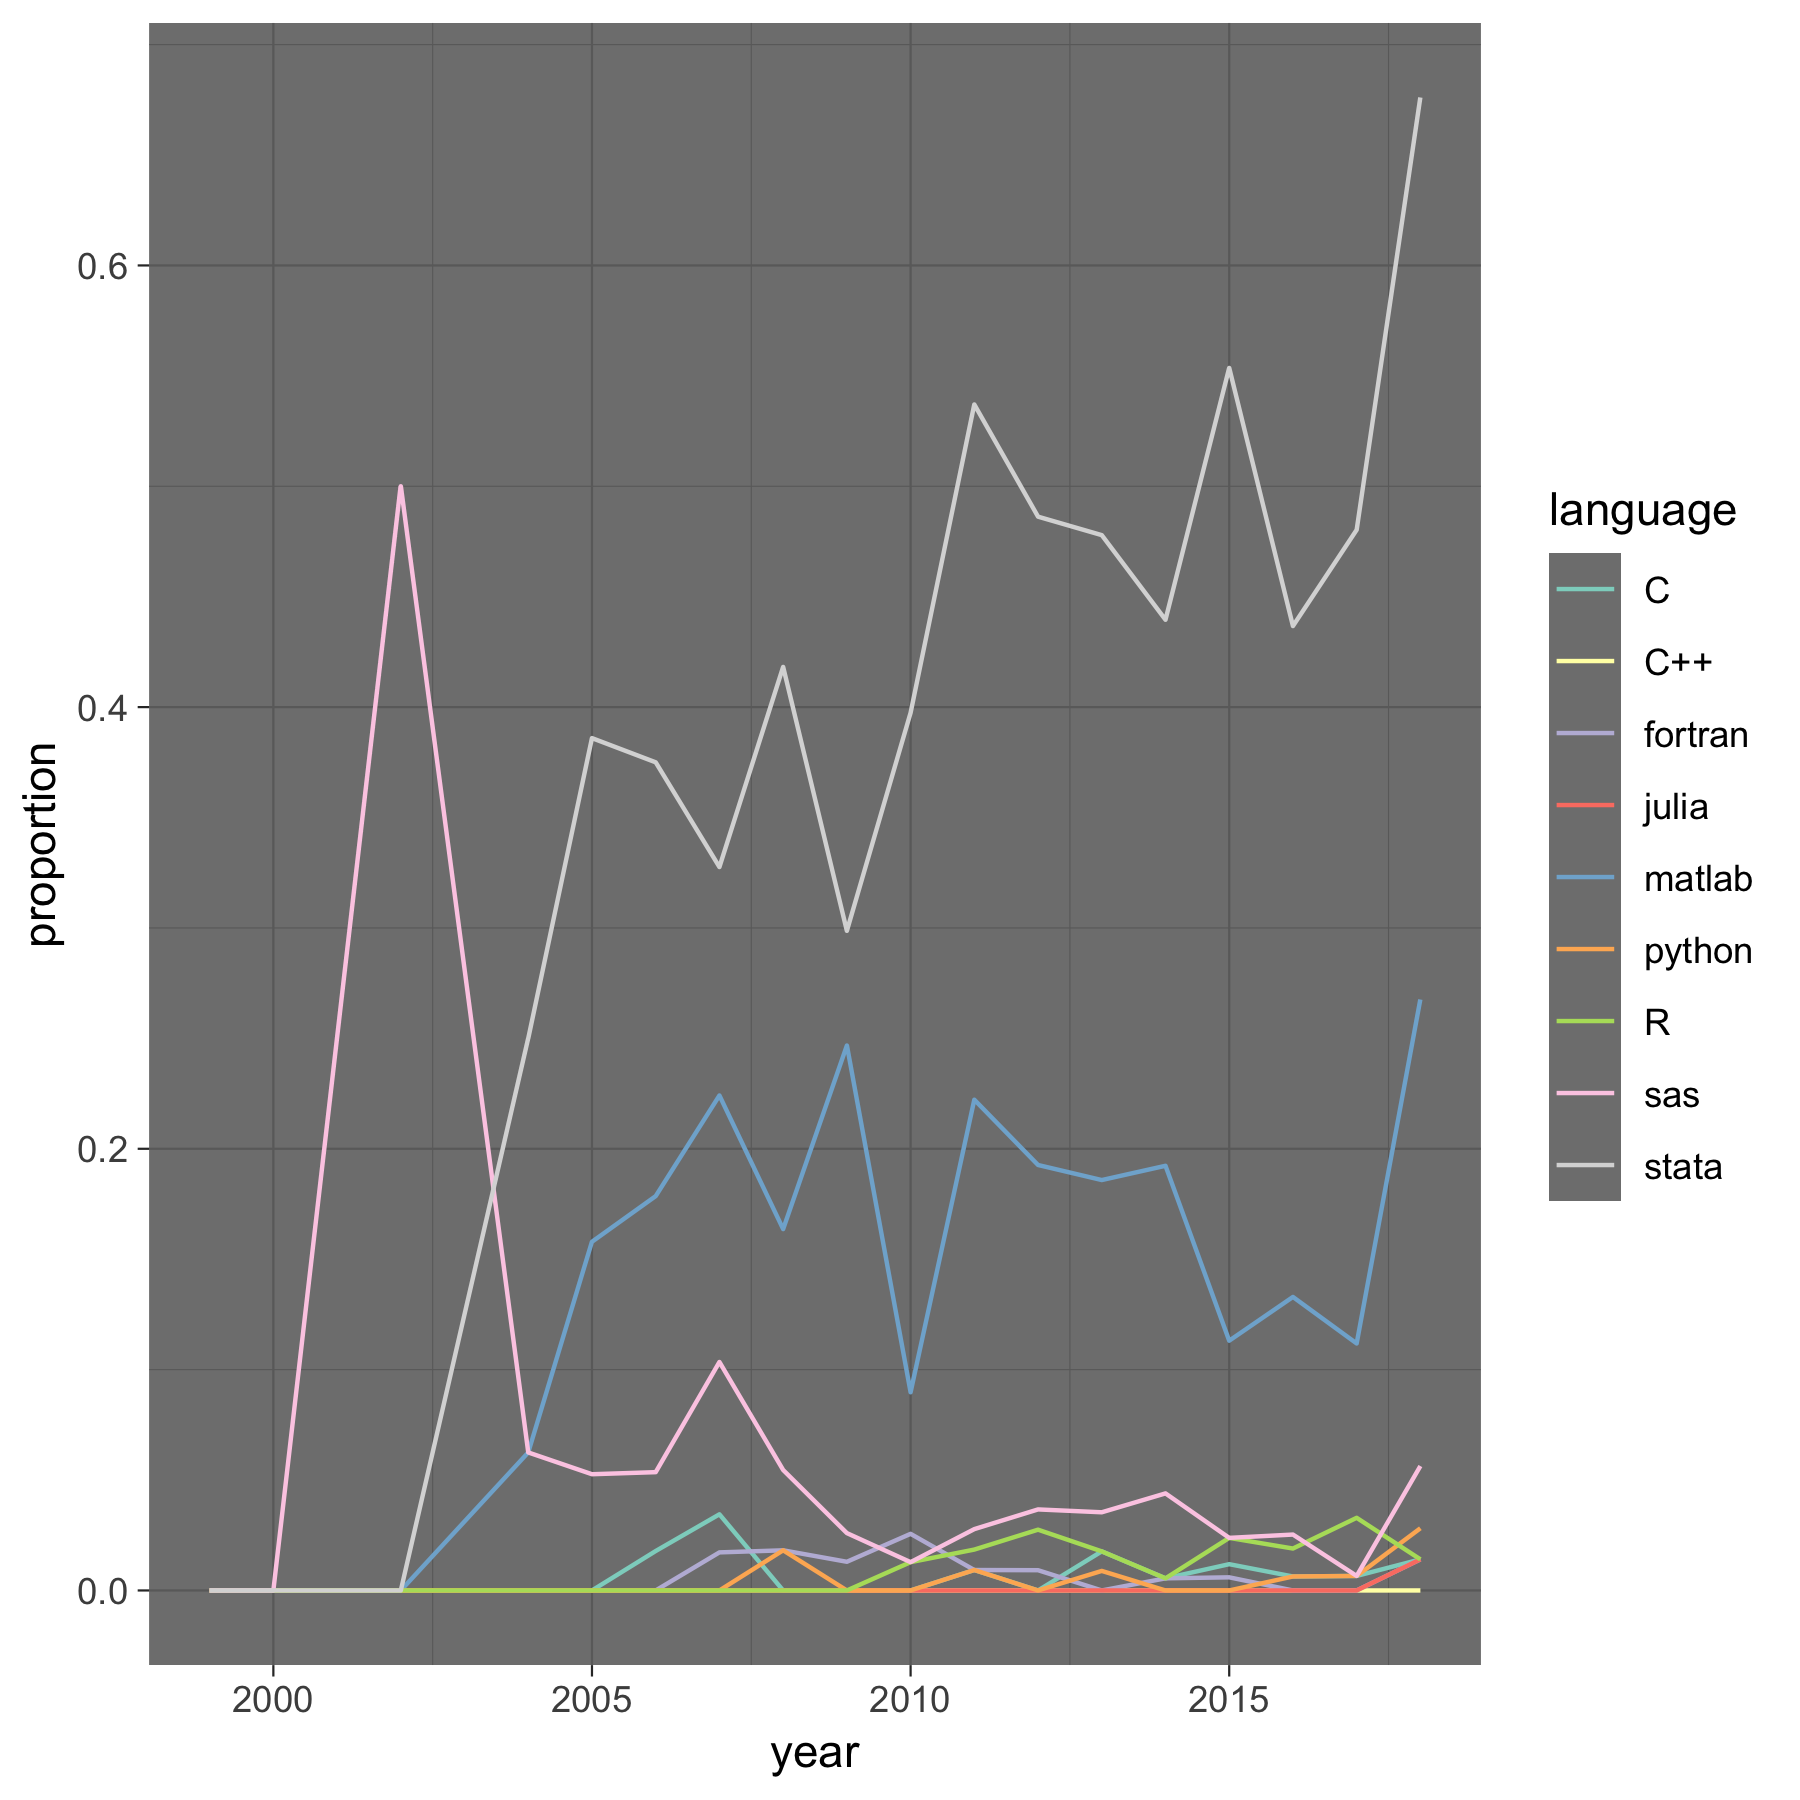
\includegraphics[width=0.45\textwidth]{images/aer_programs_by_year.png}
   
  &
    %\includegraphics[width=0.45\textwidth]{images/aejae_programs_by_year.png}
    
   \\
 AER & AEJ:AE \\
      \footnotesize Figure provided by Patrick Baylis (UBC), based on filename extensions in ZIP files of replication materials on the AEA website.\\
\end{tabular}
\caption{Popularity of statistical software\label{fig:aer_programs_by_year}}
\end{figure}

Third, we are explicitly not attempting to address data curation, though we will do simple checks for data documentation (can a reproducer understand what the file is for). Furthermore,  by allowing for third-party archives, we expect that the authors' home institutions or third parties may increasingly offer assistance with this, regardless of where the author will be submitting the article. 


\section{Task 3: Working with other providers of scientific infrastructure to improve support for documenting provenance and replicability}
We are engaging with other providers - both within the economics community, and elsewhere. 

\paragraph{Restricted-access data and verification} Naturally, given the preponderance of restricted-access data used in economics research, the verification of code that uses such data is challenging. For now, such code will not be verifiable. However, we are aware of efforts in various areas looking to provide verification services when data are restricted-access, either by third-parties with access rights, or the data providers themselves as part of their disclosure-avoidance procedures. We  are actively engaging in and supporting such efforts. We have also explored in specific cases if members of our Replication Lab might  obtain short-term access to such data, so far without success.

\paragraph{Journals} We have had discussions with members of the board of the Review of Economic Studies. The board has recently appointed a Data Editor there as well, and we look forward to collaborations. We have also discussed with editors of the Journal of Labor Economics, the Industrial and Labor Relations Review, the Journal of Human Resources, and Sociological Sciences. At conferences such as those of the Research Data Alliance (RDA) and the FORCE11 group, we have participated in workshops, forums, and one-on-one discussions with publishers (Springer Nature) and data curators, and expect to be more formally engaged in working groups in the future. 

\section{Task 4: Working with the economics community to enhance and broaden education on replicable science}

\subsection{Data Citations}
Properly referencing data goes beyond just reproducibility - it is also proper scientific writing style. In the same way that we use bibliographic references to ``printed'' resources, we should also be using such references for data resources, to give and receive credit where credit is due. Not referencing an article or book is at best an oversight, and at worst plagiarism - and the same should apply to data objects. Numerous guides and tutorials exist  \citep{dataone-l09,icpsr-data-cite,force11declaration}. However, few data citations actually occur in AEA journals.

The AEA uses the Chicago style for citations and bibliographies \citep{aeadatarefs}. However, the Chicago Style Manual \citep{citation-machine,ChicagoManualofStyleChicagoManualStyle2018} does not provide examples for data citations, and neither does the \urlcite{https://citationstyles.org/}{Citation Style Language} used by applications like \urlcite{https://www.zotero.org/}{Zotero} and \urlcite{https://www.mendeley.com/download-desktop/}{Mendeley Desktop}.%
\footnote{The object type `dataset' is defined within CSL, but not implemented in software. Zotero is expected to support an item type `dataset' as of version 5.1. In December 2018, Zotero is at version 5.0.58.}
We believe that data citations will be much more prevalent if (a) data providers consistently provide them in machine-readable formats that software can understand and (b) software can consistently provide it in the format required by the journal.

Together with the  AEA editorial office, we have   started the process of updating AEA templates available through such software.\footnote{For the technically inclined, this process involves updating an existing style or creating a new style on \url{https://citationstyles.org/} and \url{https://github.com/citation-style-language/styles}, from where it propagates to a large number of software packages.} We have also made minor adjustments to the data citation template \citep{aeadatarefs}, to conform to newer guidelines, for instance for representing \ac{DOI}.\footnote{I have also produced a draft update to the Bibtex style distributed by the AEA (\texttt{aea.bst}), see  \url{https://github.com/AEADataEditor/aea-de-guidance/blob/master/citations/aea-mod.bst} to download.}

Furthermore, for two journals, we will start monitoring data citations during the refereeing process. The \textit{Replication Lab} will do a short assessment of data used and created in articles, verify whether data citations are present, and provide a report to editors, who in turn can provide the report to authors as part of the usual editorial feedback. Authors should expect to see these reports in 2019Q1.

\section{Possible issues}
During our consultations with editors, authors, and other participants, we encountered a few possible issues worth mentioning.

\paragraph{Inability to provide information} Some authors might not be able to provide information on their data provider's preservation policies, or might not be able to provide reproducible information on data and code location when access is restricted, for instance within corporate computer networks. We have consistently iterated that the policy enforcement remains in the hands of the editor responsible for the paper. The policies above are meant to provide more information than was available in the past, including about legitimate cases where no information is available.

\paragraph{Delays} Many editors were worried that increased verification procedures might delay publication. We have attempted to address this concern by providing a flexible `trigger' for the verification procedures, by collecting information on how fast assessments and verifications can be handled, and how to scale such tasks. The most important mechanism to avoid delays in the editorial and publication workflow is to have the information about data and code as early as possible, and yet to be able to adjust the time-intensive processes to fall into periods where long delays are normal, such as during a revise-and-resubmit stage. We remain attentive to such concerns, and monitor the situation.




\section{Future activities}

\paragraph{Issuing a new data and code availability policy} Once the various activities above coalesce into solid timelines, authors, editors, and referees must be made aware of new policies. In particular, while new deposit procedures to the ``AEA Data and Code Archive'' will not materially impact the research workflow of authors, allowing for third-party repositories might impact authors, and pre-publication verification of code reproducibility will most definitely impact the way authors prepare for submission of articles. We do not wish to unduly delay submission or publication, and will therefore roll out new submission requirements (new data and code availability policies) with sufficient advance notice so authors can incorporate these into their workflow. We foresee at least two variants of a data and code availability policies (Figure~\ref{fig:policies}). Policy A.1 is the current policy, widely adopted by journals of the AEA as well as others. When introducing the ``AEA Data and Code Archive,'' the policy will need to be adapted, without fundamentally changing its intent or enforcement (Policy A.2). In particular, provision of supplemental data will be expected post-acceptance. Implementing Policy A.2, however, will involve changes to the workflow for authors, editors, and staff, and will be subject to advance notice. Each policy comes with its set of instructions  (Figure~\ref{fig:instruction}). The policies can also be compared at \url{https://docs.google.com/spreadsheets/d/1khrXxnmKC7Llj9vH17r1KEkN0hcTVqZnQloretcOwDA/edit?usp=sharing}, and comments can be sent to \url{mailto:dataeditor@aeapubs.org}. We note that the data and code availability policy itself will be curated and versioned, by publication in either the AER or the PP. Articles will have a note indicating under what policy the submission occurred. 

\begin{figure}
	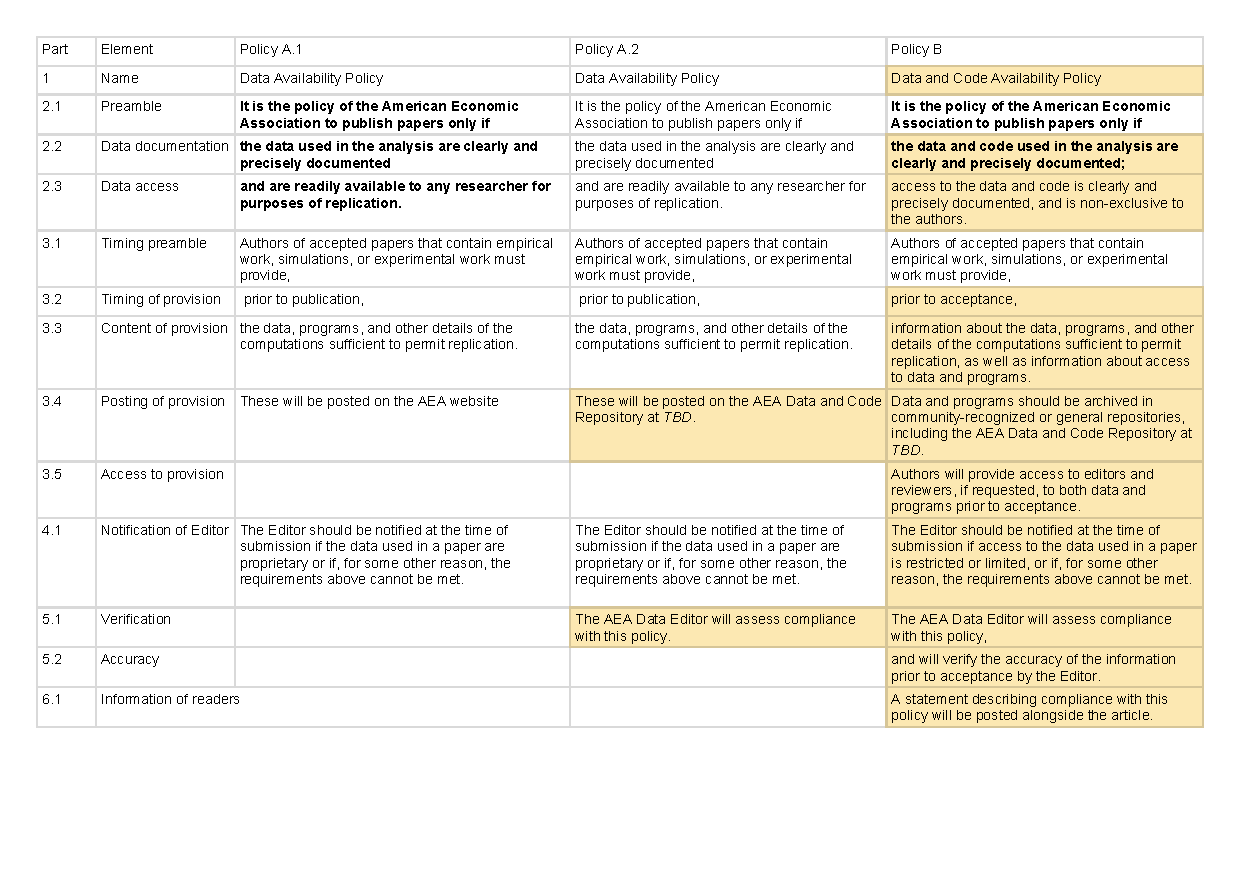
\includegraphics[width=\textwidth]{images/AEA_Data_and_Code_Availability_Policies_-_Policies.pdf}
	\caption{Proposed data and code availability policies\label{fig:policies}}
	
	\centering \footnotesize \textsc{Note:} Also available at \url{https://docs.google.com/spreadsheets/d/1khrXxnmKC7Llj9vH17r1KEkN0hcTVqZnQloretcOwDA/edit?usp=sharing}
\end{figure}
\begin{figure}
	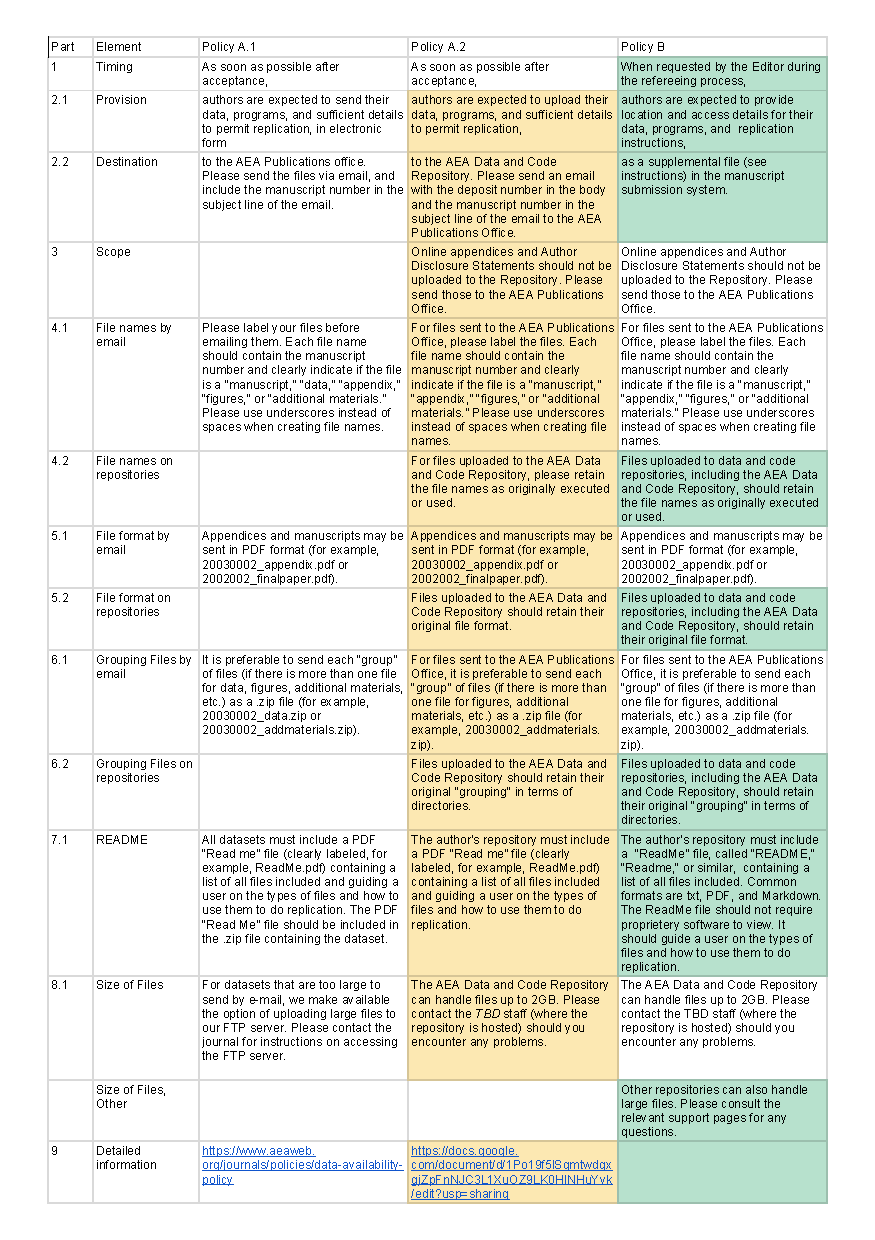
\includegraphics[width=\textwidth]{images/AEA_Data_and_Code_Availability_Policies_-_Instructions.pdf}
	\caption{Instructions for proposed data and code availability policy\label{fig:instructions}}
	
	\centering \footnotesize \textsc{Note:} Also available at \url{https://docs.google.com/spreadsheets/d/1khrXxnmKC7Llj9vH17r1KEkN0hcTVqZnQloretcOwDA/edit?usp=sharing}
\end{figure}

\paragraph{RCT}
We have spent little time this year considering the improved inclusion of \ac{RCT}. The \textit{information package} outlined above will handle better referencing of registrations, e.g. in the \urlcite{https://www.socialscienceregistry.org/}{AEA RCT Registry}. However, we will also engage with MIT to consider how the AEA RCT Registry can potentially be improved.

\paragraph{Other activities}
Furthermore, as pointed out above, we continue to engage with the research data community, while keeping abreast of  novel techniques \citep[Codeocean.com]{BrinckmanFutureGener.Comput.Syst.2018}, developments in the pre-publication phase \citep{Butler2018} and the new publication methods such as registered reports \citep{ChrisChambersReviewers'Update2014,NosekSoc.Psychol.2014}.

% Remove or comment out the next two lines if you are not using bibtex.
\bibliographystyle{aea}
\bibliography{paper,references,zotero}

% The appendix command is issued once, prior to all appendices, if any.
\appendix

\section{Replication Team}
The following members of the Replication Lab provided valuable assistance to the Data Editor in one or more of his tasks:

%first,initial,last,year
\csvreader[/csv/head=true,%
/csv/head to column names=true,%
/csv/late after line={,},%
/csv/late after last line=.,%
]%
{data/Replication_Students_Historically.csv}{}{	\first \xspace \initial \xspace \last }

\end{document}

